\section{Event rates}\label{sec:Events}

For EMRBs to be a useful astronomical signal we require that the bursts contain sufficient information to improve our knowledge of their source systems and that their event rate is sufficiently high that we could expect to observe them over a mission life time. We have addressed the first: EMRBs can give good constraints on the key parameters describing the Galaxy's MBH. The second concern shall be addressed here. Previously, the best estimate for the event rate was given by \citet{Hopman2007}; they predicted the event rate for LISA was $\sim 1\units{yr^{-1}}$. We follow a similar approach, but significantly, we improve the calculation of SNR by using NK waveforms.

\subsection{The distribution function}

We wish to calculate the probability there is an encounter between a compact object, on an orbit described by eccentricity $e$ and periapse radius $r\sub{p}$, and the MBH. We begin by following the work of \citet{Bahcall1976, Bahcall1977} and assuming the distribution function (DF) $f$ within the galactic core is only a function of the orbital energy \citep{Shapiro1978}. The energy per unit mass of the orbit is
\begin{equation}
\mathcal{E} = \frac{v^2}{2} - \frac{GM_\bullet}{r},
\end{equation}
where $v$ is orbital velocity. The number of stars is
\begin{equation}
N = \int \dd^3r \int \dd^3v f(\mathcal{E}).
\end{equation}
Close to the centre of the Galactic core, dynamics are dominated by the influence of the MBH as it is significantly more massive than the surrounding stars. Its radius of influence is \citep{Frank1976}
\begin{equation}
r\sub{c} = \frac{GM_\bullet}{\sigma^2},
\label{eq:r_c}
\end{equation}
where $\sigma^2$ is the line-of-sight velocity dispersion. We assume the mass of stars enclosed within $r\sub{c}$ is greater than the $M_\bullet$, which is much greater than the mass of a typical star $M_\star$ \citep{Bahcall1976}. We define a reference number density $n_\star$ from the enclosed mass $m_\ast(r)$ such that
\begin{equation}
m_\star(r\sub{c}) = \frac{4\pi r\sub{c}^3}{3}n_\star M_\star.
\end{equation}
Within the core, the DF can be calculated using the approximation of Fokker-Planck formalism \citep[section 7.4]{Binney2008}. The population of bound stars is evolved numerically until a steady state is reached: the unbound stars form a reservoir with an assumed Maxwellian distribution. Denoting a species of star by its mass $M$,
\begin{equation}
f_M(\mathcal{E}) = \frac{C_M n_\star}{(2\pi\sigma_M^2)^{3/2}} \exp\left(-\frac{\mathcal{E}}{\sigma_M^2}\right),\quad\mathcal{E} > 0,
\label{eq:Unbound_DF}
\end{equation}
where $C_M$ is a normalisation constant.\footnote{$C_M$ determines the population ratios of species $M$ far from the black hole \citep{Alexander2009}.} If different stellar species are in equipartition, as assumed by \citet{Bahcall1976, Bahcall1977}, we expect
\begin{equation}
M \sigma_M^2 = M_\star \sigma_\star^2.
\end{equation}
However, if the unbound stellar population has reached equilibrium by violent relaxation, all mass groups are expected to have similar dispersions:
\begin{equation}
\sigma_M = \sigma_\star = \sigma,
\end{equation}
and we have equipartition of energy per unit mass \citep{Lynden-Bell1967}. This is assumed here following \citet{Alexander2009} and \citet{O'Leary2009}. The steady-state DF is largely insensitive to this choice \citep{Bahcall1977, Alexander2009}.

For bound orbits, the DF can be approximated as a power law \citep{Peebles1972}
\begin{equation}
f_M(\mathcal{E}) = \frac{k_M n_\star}{(2\pi\sigma^2)^{3/2}}\left(-\frac{\mathcal{E}}{\sigma^2}\right)^{p_M},\quad\mathcal{E} < 0.
\label{eq:Bound_DF}
\end{equation}
The exponent $p_M$ varies depending upon the mass of the object, determining mass segregation. For a system with a single mass component $p = 1/4$ \citep{Bahcall1976, Young1977}. The normalisation constant $k_M$ reflects the relative abundances of the different species.\footnote{For a single mass population ($p = 1/4$) $k = 2 C$ gives a fit correct to within a factor of two \citep{Bahcall1976,Keshet2009}, we assume this holds for the dominant species of stars as, although it changes slightly with $p$, variation is small compared to errors introduced by fitting a simple power law \citep{Hopman2006, Alexander2009}.}

These cusp profiles should exist if the system has had sufficient time to become gravitationally relaxed. There is current debate about whether this may be the case, both for the Galactic centre and galaxies in general. This is discussed further in \apref{tauGC}. For concreteness, we assume a cusp has formed. If a cusp has not formed, we expect there to be a shallower core profile, with fewer objects passing close to the MBH. Our results are therefore an upper bound on possible event rates \citep{Merritt2010a,Gualandris2012}. 

\subsection{Model parameters}\label{sec:GC-Param}

We use the Fokker-Planck model of \citet{Hopman2006, Hopman2006a, Alexander2009}. This includes four stellar species: main sequence (MS) stars, white dwarfs (WDs), neutron stars (NSs), and black holes (BHs). Their properties are summarised in \tabref{HA}. The behaviour of the Fokker-Planck model has been verified by $N$-body simulations \citep{Baumgardt2004,Preto2010}.
\begin{table}[!htp]
 \centering
  \begin{tabular}{l D{.}{.}{2.1} D{.}{.}{1.3} D{.}{.}{1.1} D{.}{.}{1.3}}
  \toprule
   Star & \multicolumn{1}{c}{$M/M_\odot$} & \multicolumn{1}{c}{$C_M/C_\star$} & \multicolumn{1}{c}{$p_M$} & \multicolumn{1}{c}{$k_M/k_\star$} \\
 \midrule
 MS & 1.0 & 1 & -0.1 & 1 \\
 WD & 0.6 & 0.1 & -0.1 & 0.09 \\
 NS & 1.4 & 0.01 & 0.0 & 0.01  \\
 BH & 10 & 0.001 & 0.5 & 0.008 \\
\bottomrule
\end{tabular}
\caption{Stellar model parameters for the Galactic core using the results of \citet{Alexander2009} We use the main sequence star as our reference. The number fractions for unbound stars are estimates corresponding to a model of continuous star formation \citep{Alexander2005}; \citet{O'Leary2009} arrive at the same proportions. Values for $k_M/k_\star$ are taken from \citet{Toonen2009}.\label{tab:HA}}
\end{table}
The steeper power law for black holes means they segregate about the MBH.\footnote{Extrapolating, they would dominate in place of MS stars for radii $r < 10^{-4}r\sub{c}$.}

Binaries may form in the galactic centre, encouraged by its high stellar density \citep{O'Leary2009}. However the binary fraction is still expected to be small \citep{Hopman2009}. Binaries are also disrupted by the MBH for periapses smaller than
\begin{equation}
r\sub{B}  \simeq \left(\frac{M_\bullet}{M_1 + M_2}\right)^{1/3}a\sub{B},
\end{equation}
where $M_1$ and $M_2$ are the masses of the binary's components, and $a\sub{B}$ is the binary's semi-major axis, cf.\ \eqnref{Tidal} below. Thus, we ignore the possible presence of binaries.

We assume $M_\bullet = (4.31 \pm 0.36) \times 10^6 M_\odot$ \citep{Gillessen2009} and $\sigma = (103 \pm 20)\units{km\,s^{-1}}$ \citep{Tremaine2002}. This gives a core radius of $r\sub{c} = (1.7 \pm 0.7)\units{pc}$. Using the results of \citet{Ghez2008} we would expect the total mass of stars core to be $m_\star(r\sub{c}) = 6.4 \times 10^6 M_\odot$, which is within $5\%$ of the value obtained similarly from \citet{Genzel2003}. This gives a reference stellar density of $n_\star = 2.8 \times 10^5\units{pc^{-3}}$.

\subsection{Parametrizing in terms of eccentricity \& periapsis}

We characterise orbits by their eccentricity $e$ and periapse radius $r\sub{p}$. The latter, unlike the semimajor axis, is always well defined regardless of eccentricity. For Keplerian orbits, the energy $\mathcal{E}$ and angular momentum $\mathcal{J}$ per unit mass are entirely characterised by these parameters
\begin{align}
\label{eq:Energy_ecc}
\mathcal{E} = {} & -\frac{GM_\bullet(1 - e)}{2r\sub{p}}; \quad \mathcal{J}^2 = GM_\bullet(1 + e)r\sub{p}.
\end{align}
The DF is defined per element of phase space: it is necessary to change variables from position and velocity to eccentricity and periapsis. We decompose the velocity into three orthogonal components: radial $v_r$, azimuthal $v_\phi$ and polar $v_\theta$. We assume the core is spherically symmetric \citep{Genzel2003, Schodel2007}, therefore we are only interested in the combination
\begin{equation}
v_\perp^2 = v_\phi^2 + v_\theta^2 = v^2 - v_r^2.
\end{equation}
Under this change of variables
\begin{equation}
\dd^3v = \dd v_r \dd v_\phi \dd v_\theta \rightarrow 2\pi v_\perp \,\dd v_r \,\dd v_\perp.
\end{equation}
The specific energy and angular momentum are given by
\begin{align}
\mathcal{E} = {} & \frac{v_r^2 + v_\perp^2}{2} - \frac{GM_\bullet}{r}; \quad \mathcal{J}^2 = r^2 v_\perp^2.
\end{align}
Combining these with our earlier expressions in terms of $e$ and $r\sub{p}$,
\begin{subequations}
\begin{align}
v_\perp^2 = {} & \frac{GM_\bullet(1 + e)r\sub{p}}{r^2}, \\*
v_r^2 = {} & GM_\bullet\left[\frac{2}{r} - \frac{(1 - e)}{r\sub{p}} - \frac{(1 + e)r\sub{p}}{r^2}\right].
\end{align}
\end{subequations}
From the latter we can verify the turning points of an orbit occur at
\begin{equation}
r = r\sub{p}, \: \frac{1+e}{1-e}r\sub{p};
\end{equation}
the periapse is the only turning point for orbits with $e > 1$. Since we now have expressions for $\{v_r, v_\perp\}$ in terms of $\{e, r\sub{p}\}$, we can 
%calculate the Jacobian
%\begin{equation}
%\left|\frac{\partial(v_r, v_\perp)}{\partial(e, r\sub{p})}\right| = \recip{2v_rv_\perp}\frac{e}{r\sub{p}}\left(\frac{GM_\bullet}{r}\right)^2.
%\end{equation}
%Using this, we may
rewrite our velocity element as
\begin{equation}
\dd^3v \rightarrow \frac{\pi e}{v_rr\sub{p}}\left(\frac{GM_\bullet}{r}\right)^2\,\dd e \,\dd r\sub{p}.
\end{equation}
As a consequence of our assumed spherical symmetry, 
%the volume element is
%\begin{equation}
%\dd^3r = 4\pi r^2 \,\dd r.
%\end{equation}
%Thus, 
the phase space volume element can be expressed as
\begin{equation}
\dd^3r\dd^3v \rightarrow \frac{4\pi^2(GM_\bullet)^2e}{v_rr\sub{p}}\,\dd r\,\dd e \,\dd r\sub{p}.
\end{equation}
The number of stars in an element $\dd r\,\dd e\,\dd r\sub{p}$ is
\begin{equation}
n(r, e, r\sub{p}) = \frac{4\pi^2(GM_\bullet)^2e}{v_rr\sub{p}}f(\mathcal{E}).
\end{equation}

From this, we can construct the expected number of stars on orbits defined by $\{e, r\sub{p}\}$. We define this locally, allowing it to vary with position. The number of stars found in a small radius range $\delta r$ with given orbital properties is
\begin{equation}
n(r, e, r\sub{p})\delta r = N(e, r\sub{p}; r)\frac{\delta t}{P(e, r\sub{p})},
\end{equation}
where $N(e, r\sub{p}; r)$ is the total number of stars with orbits given by $\{e, r\sub{p}\}$ defined at $r$, $\delta t$ is the time spent in $\delta r$ and $P(e, r\sub{p})$ is the period of the orbit. We defer the definition of this time for unbound orbits for now. The time spent in the radius range is
\begin{equation}
\delta t = 2\frac{\delta r}{v_r},
\end{equation}
where the factor of $2$ accounts for inwards and outwards motion. Hence
\begin{align}
N(e, r\sub{p}; r) = {} & \recip{2} v_r P(e, r\sub{p}) n(r, e, r\sub{p}) = \frac{2\pi^2(GM_\bullet)^2 e P(e, r\sub{p})}{r\sub{p}}f(\mathcal{E}).
\end{align}
The right hand side is independent of position, subject to the constraint that the radius is in the allowed range for the orbit $r\sub{p} \leq r \leq (1+e)r\sub{p}/(1-e)$, and so $N(e, r\sub{p}) \equiv N(e, r\sub{p}; r)$. This is a consequence of the DF being dependent only upon a constant of the motion.\footnote{See \citet{Bahcall1976} equation (9) for a similar result.}

If a burst of radiation is emitted each time a star passes through periapse, the event rate for burst emission from orbits with parameters $\{e, r\sub{p}\}$ is given by
\begin{align}
\Gamma(e, r\sub{p}) = {} & \frac{N(e, r\sub{p})}{P(e, r\sub{p})} = \frac{2\pi^2(GM_\bullet)^2 e}{r\sub{p}}f(\mathcal{E}).
\label{eq:Gamma}
\end{align}
The orbital period drops out from the calculation, so we do not have to worry about an appropriate definition for unbound orbits.

%From the event rate we may define a probability of seeing a given number of events subject to the assumption they are uncorrelated: it is given by the Poisson distribution. The probability of there being $r$ events is
%\begin{equation}
%\Pr(r|\Gamma(e, r\sub{p})) = \frac{\Gamma^r\exp(-\Gamma)}{r!}.
%\end{equation}
%The probability of there being a burst from an orbit with periapse $r\sub{p}$ and eccentricity $e$ is hence
%\begin{equation}
%\Pr(r \neq 0|\Gamma(e, r\sub{p})) = 1 - \Pr(r = 0|\Gamma(e, r\sub{p})).
%\end{equation}

%To estimate the expectation of a quantity across all orbits we use
%\begin{equation}
%\left\langle X\right\rangle = \sum\sub{R} \int_0^\infty \dd e \int_0^\infty \dd r\sub{p} X(r;r\sub{p},e)\Pr(r|\Gamma(e, r\sub{p})).
%\end{equation}
%Since the probability decays rapidly for large $r$, we may truncate the sum to give the required level of accuracy,

To generate a representative sample for the orbital parameters $e$ and $r\sub{p}$, we use $\Gamma(e, r\sub{p})\dd e\, \dd r\sub{p}$ as the rate for a Poisson distribution.

\subsection{The inner cut-off}

From \eqnref{Gamma} we see the event rate is highly sensitive to the smallest value of the periapsis. Ultimately the orbits cannot encroach closer to the MBH than its last stable orbit. This depends upon the spin of the MBH, but is of the order of its Schwarzschild radius. Before we reach this point, there are other processes that may intervene to deplete the orbiting stars. Our treatment of these is approximate, but should produce reasonable estimates. We consider three processes: tidal disruption by the MBH; GW inspiral, and collisional disruption. Tidal disruption imposes a definite (albeit approximate) cut-off, while the others use statistical arguments. For these methods, we will need to define a reference time-scale for relaxation which is done in \secref{Relax}, with further details found in \apref{time-scale}.

The calculated inner cut-offs for the four stellar species are shown in \figref{Cuts}.
\begin{figure}[!htp]
\begin{center}
   \subfigure[{Main sequence stars}]{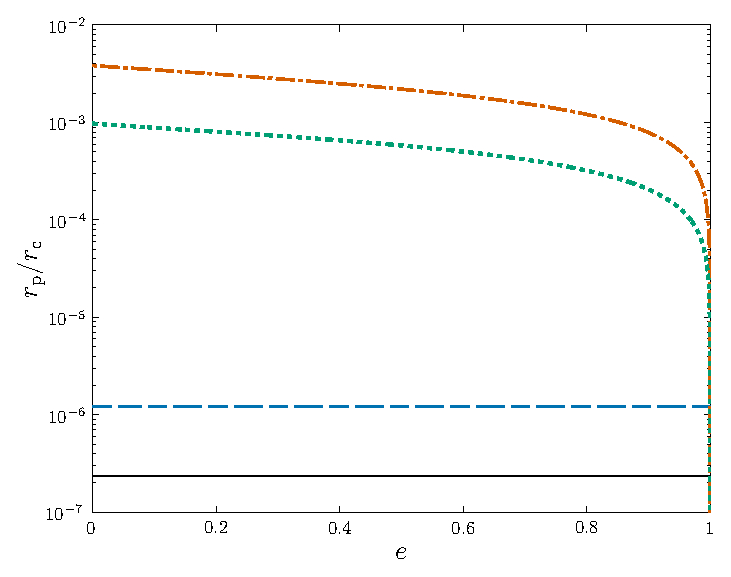
\includegraphics[width=0.45\textwidth]{./images/Fig_Inner_cut_1.eps}} \quad 
   \subfigure[{White dwarfs}]{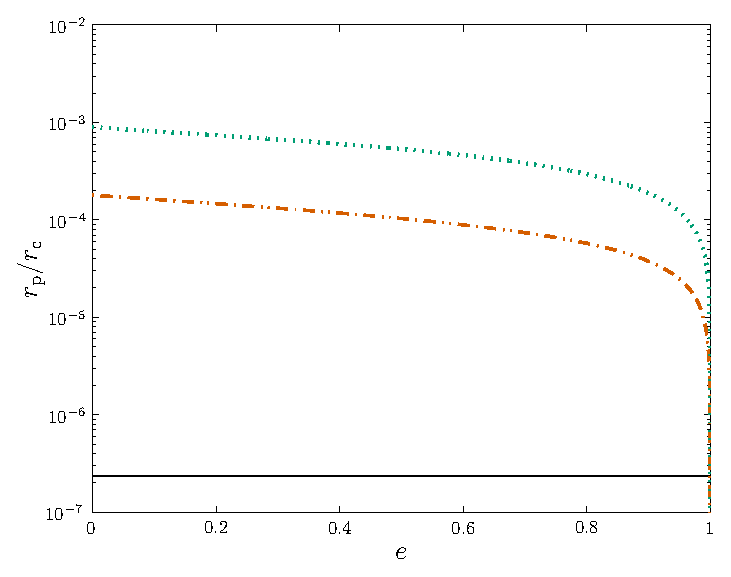
\includegraphics[width=0.45\textwidth]{./images/Fig_Inner_cut_2.eps}} \\
   \subfigure[{Neutron stars}]{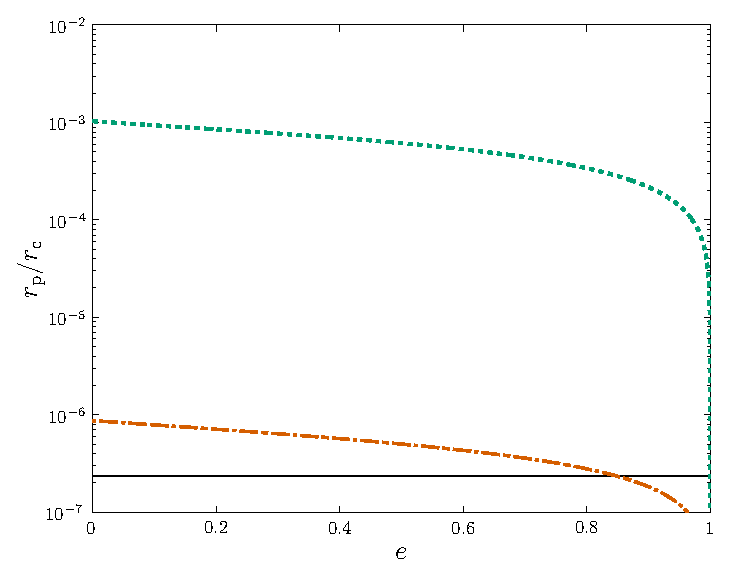
\includegraphics[width=0.45\textwidth]{./images/Fig_Inner_cut_3.eps}} \quad
   \subfigure[{Black holes}]{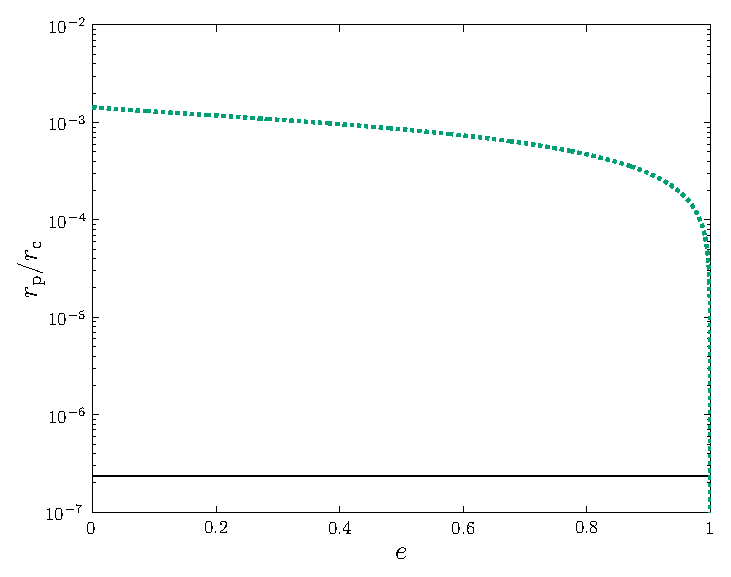
\includegraphics[width=0.45\textwidth]{./images/Fig_Inner_cut_4.eps}}
\caption{Inner cut-off radii as a function of eccentricity. The solid line is the Schwarzschild radius of the MBH; the dashed line is the tidal radius; the dot-dashed line is the collisional cut-off, and the dotted line is the transition to the GW-dominated inspiral regime.\label{fig:Cuts}}
  \end{center}
\end{figure}

\subsubsection{Tidal disruption}

Tidal forces from the MBH can disrupt stars. This occurs at the tidal radius
\begin{equation}
r\sub{T} \simeq \left(\frac{M_\bullet}{M}\right)^{1/3}R_M
\label{eq:Tidal}
\end{equation}
where $R_M$ is the radius of the star \citep{Hills1975, Rees1988, Kobayashi2004}.\footnote{See \citet{Kesden2012} for a general relativistic treatment.} Any star on an orbit with $r\sub{p} < r\sub{T}$ is disrupted in the course of its orbit. Parametrizing orbits by their periapsis allows us to easily determine which stars should be disrupted. We do not include the full effects of the loss cone \citep{Frank1976, Lightman1977, Cohn1978} as these were not incorporated into the Fokker-Planck calculations \citep{Hopman2009}.\footnote{The loss cone is a region in velocity space where orbits are depleted because stars are disrupted more rapidly than they can be replenished by two-body scattering.} The effect of the loss cone should be small, only modifying the DF by a logarithmic term \citep{Lightman1977, Bahcall1977, Cohn1978}. Its effects are diluted by resonant relaxation \citep{Hopman2007,Toonen2009,Merritt2011}. Furthermore, the loss cone could be refilled by the wandering of the MBH because of perturbations from the inhomogeneities in the stellar potential \citep{Sigurdsson1997,Chatterjee2002,Merritt2007}.

Tidal disruption is significant for MS stars since they are least dense: calculated in this way, only MS stars are tidally disrupted outside of the MBH's event horizon \citep{Sigurdsson1997}. The tidal radius defines the cut-off for periapsis of high eccentricity ($e \gtrsim 1$) orbits \citep{Lightman1977}.

\subsubsection{Relaxation time-scale}\label{sec:Relax}

The motion of a star is determined not only by the dominant influence of the central MBH, but also by the other stars. The gravitational potential of the stars may be split into two components: a smooth background representing the average distribution of stars, and statistical fluctuations from random deviations in the stellar distribution. The former only contributes to the stars' orbits: we neglect this since we are more interested in the influence of the MBH. The latter may be approximated as a series of two-body encounters. These lead to scattering, in a manner much like Brownian motion \citep{Bekenstein1992,Maoz1993,Nelson1999}.

The two-body interactions mostly lead to small deflections. Over time, these may accumulate into a significant change in the dynamics. The relaxation time-scale characterises the time taken for this to happen \citep[section 1.2.1]{Binney2008}. It therefore quantifies the time over which an orbit may be repopulated by scattering. There are a variety of definitions for the relaxation time-scale. For a system with a purely Maxwellian distribution, the time-scale has form
\begin{equation}
\tau\sub{R}\super{Max} \simeq \kappa\frac{\sigma^3}{G^2M_\star^2 n_\star\ln\Lambda},
\label{eq:tauMaxwell}
\end{equation}
where the Coulomb logarithm is $\ln\Lambda = \ln(M_\bullet/M_\star)$ \citep{Bahcall1976}, and $\kappa$ is a dimensionless number. In his pioneering work, \citet{Chandrasekhar1941, Chandrasekhar1960} defined the time-scale as the period over which the squared change in energy was equal to the kinetic energy squared, this gives $\kappa = 9/16\sqrt{\pi} \simeq 0.32$. Subsequently, \citet{Chandrasekhar1941a} described relaxation statistically, treating fluctuations in the gravitational field probabilistically; this gives $\kappa = 9/2(2\pi)^{3/2} \simeq 0.29$. \citet{Bahcall1977} define a reference time-scale from their Boltzmann equation with $\kappa = 3/4\sqrt{8\pi} \simeq 0.15$; this is equal to the reference time-scale defined as the reciprocal of the coefficient of dynamical friction by \citet{Chandrasekhar1943a, Chandrasekhar1943}. \citet{Spitzer1958} define a reference time-scale from the gravitational Boltzmann equation of \citet{Spitzer1951} where $\kappa = \sqrt{2}/\pi \simeq 0.45$. Following \citet{Spitzer1971}, \citet[section 7.4.5]{Binney2008} estimate the time-scale from the velocity diffusion coefficient of the Fokker-Planck equation yielding $\kappa \simeq 0.34$.

All these approaches yield consistent values, suggesting, as a first approximation, any is valid. We follow the classic treatment of \citet[chapter 2]{Chandrasekhar1960} which is transparent in its assumptions, adapting from a Maxwellian distribution of velocities to one derived from the DFs (\ref{eq:Unbound_DF}) and (\ref{eq:Bound_DF}). This makes the model self-consistent. Since there is uncertainty in the astrophysical parameters, we will not be concerned by small discrepancies in the numerical prefactor that result from the simplifying approximations of this approach. Whilst we are only making a minor change to the derivation of the relaxation time-scale, the calculations become much more involved; we confine this to \apref{time-scale}, along with a discussion of the shortcomings. An average time-scale for the entire system $\overline{\tau\sub{R}}$ is defined in \eqnref{system-relax}, and an average for an orbit $\left\langle\tau\sub{R}\right\rangle$ is defined in \eqnref{orbital-relax}.

Two-body interactions lead to diffusion in both energy and angular momentum. When considering a single (bound) orbit, over a relaxation time-scale the energy changes by order of itself while the angular momentum changes by the angular momentum of a circular orbit with that energy $\mathcal{J}\sub{circ}(\mathcal{E})$ \citep{Lightman1977, Rauch1996, Hopman2005, Madigan2011}:\footnote{$\mathcal{J}\sub{circ}(\mathcal{E})$ is the maximum value for orbits of that energy.}
\begin{equation}
\left(\frac{\Delta\mathcal{E}}{\mathcal{E}}\right)^{2} \approx \left[\frac{\Delta \mathcal{J}}{\mathcal{J}\sub{circ}(\mathcal{E})}\right]^{2} \approx \frac{t}{\tau\sub{R}}.
\label{eq:diffuse-relax}
\end{equation}
We may define another angular momentum relaxation time-scale as the time taken for the angular momentum to change by order of itself \citep{Merritt2011}
\begin{align}
\tau_\mathcal{J} = {} & \left[\frac{\mathcal{J}}{\mathcal{J}\sub{circ}(\mathcal{E})}\right]^2\tau\sub{R} = \left(1 - e^2\right) \tau\sub{R}.
\label{eq:J-time}
\end{align}
This can be much shorter than the energy relaxation time-scale: diffusion in angular momentum can proceed more rapidly than diffusion in energy.

\subsubsection{Gravitational wave inspiral}\label{sec:GW-in}

Stars orbiting the MBH continually emit gravitational radiation; this carries away energy and angular momentum, causing the stars to inspiral. Using the analysis of \citet{Peters1963} and \citet{Peters1964} for Keplerian binaries, it is possible to define a characteristic inspiral time-scale from the rate of change of energy. For consistency with the relaxation time-scale, we define this as \citep{MiraldaEscude2000, Merritt2011}
\begin{equation}
\tau\sub{GW} \simeq \mathcal{E}\left\langle\diff{\mathcal{E}}{t}\right\rangle^{-1},
\label{eq:tGW-def}
\end{equation}
where the term in angular brackets is the orbit-averaged rate of energy radiation. Using \eqnref{Energy_ecc} and equation (16) of \citet{Peters1963},
\begin{align}
\tau\sub{GW} \simeq {} & \frac{5}{64}\frac{c^5r\sub{p}^4}{G^3MM_\bullet\left(M + M_\bullet\right)}\frac{(1+e)^{7/2}}{(1-e)^{1/2}} \left(1+\frac{73}{24}e^2 + \frac{37}{96}e^4\right)^{-1} \\
 \approx {} & \frac{5}{64}\frac{c^5r\sub{p}^4}{G^3MM_\bullet^2}\frac{(1+e)^{7/2}}{(1-e)^{1/2}}\left(1+\frac{73}{24}e^2 + \frac{37}{96}e^4\right)^{-1}.
\end{align}
The characteristic time-scale is a better measure of the depletion of an orbit than the total inspiral time as it only depends upon the parameters of that orbit, and not its future evolution.

The time-scale associated with changes in angular momentum is \citep{Peters1964}
\begin{align}
\tau_{\mathrm{GW},\, \mathcal{J}} \simeq {} & \mathcal{J}\left\langle\diff{\mathcal{J}}{t}\right\rangle^{-1} \\
 \simeq {} & \frac{5}{32}\frac{c^5r\sub{p}^4}{G^3MM_\bullet\left(M + M_\bullet\right)}\frac{(1+e)^{5/2}}{(1-e)^{3/2}}\left(1+\frac{7}{8}e^2\right)^{-1} \\
 \approx {} & \frac{5}{32}\frac{c^5r\sub{p}^4}{G^3MM_\bullet^2}\frac{(1+e)^{5/2}}{(1-e)^{3/2}}\left(1+\frac{7}{8}e^2\right)^{-1}.
\end{align}
This is always greater than the energy time-scale; hence, we only consider changes in energy from GW emission as important for evolution of the system \citep{Hopman2005}.

Unbound stars only undergo a single periapse passage and only radiate one burst of radiation; we therefore neglect any evolution in their orbital parameters.\footnote{Changes are only important for very high eccentricity orbits. These are very high energy, and exponentially suppressed because of the Boltzmann factor in \eqnref{Unbound_DF}.}

The $(1-e)^{-1/2}$ dependence of $\tau\sub{GW}$ for bound orbits connects the two regimes. The rate of change of energy goes to zero as a consequence of assuming the orbital parameters do not change over the course of an orbit. It is a valid approximation since the large mass-ratio ensures a slow evolution of the system.

When comparing with the relaxation time-scale we are comparing rates of change, with the shorter time-scale highlighting the more rapid process that dominates the evolution \citep{Amaro-Seoane2007}. We therefore compare $\tau\sub{GW}$ with the orbital relaxation time-scale $\tau_\mathcal{J}$ \citep{Merritt2011}. Orbits with $\tau\sub{GW} < \tau_\mathcal{J}$ become depleted by GW emission faster than they are replenished by scattering. The cusp does not extend to these orbits. Yet, these orbits are not totally depopulated as an object may pass through during its inspiral from greater periapse and eccentricity. The net effect is the distributions of MS stars, WDs and NSs at high eccentricities are relatively unchanged from their cusp states, but the BH population is significantly depleted.

\subsubsection{Collisions}\label{sec:Collision}

As a consequence of the high densities in the Galactic core, stars may undergo a large number of close encounters with other stars \citep{Cohn1978}. These may lead to their destruction. MS stars, WDs, and NSs may be pulled apart by tidal forces if they stray too close to a more massive object. As MS stars are diffuse, they would not tidally disrupt another star \citep{Murphy1991,Freitag2005}. Close encounters would result in some mass transfer; the cumulative effect of $20$--$30$ grazing collisions could destroy a MS star \citep{Freitag2006}. The number of collisions a star undergoes in a time interval $\delta t$ is
\begin{equation}
\delta K = n(r) A v(r,e,r\sub{p})\delta t,
\end{equation}
where $A$ is the collisional cross-sectional area. For tidal disruption, where the encounter is with a collapsed object (WD, NS or BH), we set $A = \pi r_{\mathrm{T},\,{M'}}^2$, where $r_{\mathrm{T},\,{M'}}$ is the appropriate tidal radius: like \eqnref{Tidal} but with $M_\bullet$ replaced with the mass of the collapsed object $M'$. For collisions between MS stars, the cross-sectional area is simply the geometric $A = \pi R_\star^2$.\footnote{Here we assume the relative velocity of the colliding stars is much greater than the escape velocity of the star so we may neglect the effects of gravitational focusing.}

For circular orbits we can find the radius at which collisions lead to disruptions by setting $\delta K = 1$ for tidal disruption or $\delta K = 20$ for grazing collisions, and $\delta t = \overline{\tau_\mathrm{R,\,M}}$. We use the system average relaxation time-scale for species of mass $M$ as this is the time over which stars are replenished from the reservoir. For non-circular orbits we must consider variation with position. Using $\delta r = v_r \delta t$, and then converting to an integral, for bound orbits
\begin{equation}
K = 2 A \frac{\tau\sub{R}}{P(r\sub{p},e)}\intd{r\sub{p}}{(1+e)r\sub{p}/(1-e)}{n(r)\frac{v(r,e,r\sub{p})}{v_r(r,e,r\sub{p})}}{r},
\end{equation}
where $P$ is the period of the orbit. Again we set $K = 1$ or $K = 20$ to find the orbits for which stars will be disrupted within $\overline{\tau_\mathrm{R,\,M}}$. For unbound orbits we are only interested in stars that would become disrupted before their periapse passage, so
\begin{equation}
K = A \intd{r\sub{p}}{r\sub{c}}{n(r)\frac{v(r,e,r\sub{p})}{v_r(r,e,r\sub{p})}}{r},
\end{equation}
assuming the stars in the reservoir external to the core are unlikely to undergo close collisions.

Collisions provide the cut-off for bound MS stars, and are significant for bound WDs.

\subsection{Number of events}

To estimate the number of events expected in a $2\units{yr}$ mission lifetime $\mathcal{N}_2$, we performed $16000$ mission realisations. For each, we randomly selected a set of parameters to describe the MBH, and then picked orbits with probabilities defined by their event rates. The lower bound on eccentricity was set to $0.9$, below which we do not trust the parabolic approximation for burst waveforms; since the DF decays exponentially with eccentricity for unbound orbits, the upper limit does not influence our results. The SNR of the resulting bursts were calculated (with the detector in a position corresponding to a random time), and a detection was recorded if $\rho > 10$. By averaging the number of events per mission, we can estimate the expected number of bursts we would expect to detect.

The calculated numbers of events are given in \tabref{Rates}.
\begin{table}[!htp]
 \centering
  \begin{tabular}{l D{,}{\times}{3.4}}
  \toprule
   Star & \multicolumn{1}{c}{$\mathcal{N}_2$} \\
 \midrule
 MS & 1.0,10^{-3} \\
 WD & 9.9,10^{-3} \\
 NS & 5.0,10^{-1} \\
 BH & 1.2,10^{0} \\
\midrule
Total & 1.7,10^{0}\\
\bottomrule
\end{tabular}
  \caption{Expected number of detectable EMRBs for a two year mission.\label{tab:Rates}}
\end{table}
The overall rates are similar to those presented in \citet{Hopman2007}. The MS rate is lower because of a larger collisional cut-off, which also influences the WD rate; the NS rate is enhanced because of the inclusion of bursts from inspiralling objects. The physics for BHs is least changed, the (small) difference in event rate is partly a consequence of our more realistic SNRs. Only MS stars have a non-negligible (relative) contribution from unbound orbits.

The number of events per mission is plotted in \figref{Event-no}.
\begin{figure}[!htp]
\begin{center}
   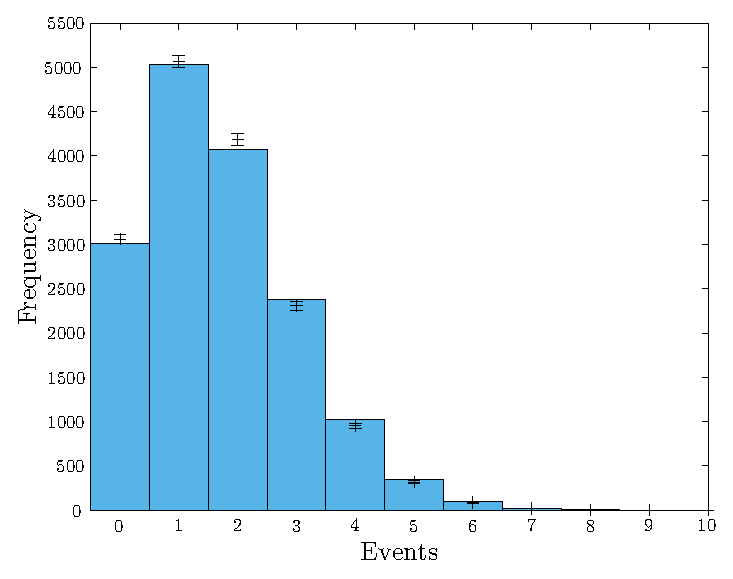
\includegraphics[width=0.6\textwidth]{./images/Fig_Total_event_hist}
\caption{Calculated number of detectable EMRBs over a two year mission. The histogram shows the number of events for 16000 realisations. The points show a Poisson distribution for the same number of missions with a mean set by integrating the event rate.}
\label{fig:Event-no}
\end{center}
\end{figure}
As a consistency check, we also calculated the expected number of bursts by numerically integrating the event rate. The lower limit on $r\sub{p}$ was set to be the largest of the tidal cut-off, the collisional cut-off or the MBH's Schwarzschild radius; the upper limit was the detection threshold as determined from \eqnref{SNR-power-law}. This gives an expectation of $\mathcal{N}_2 \simeq 1.7$ in good agreement with our other estimate. We have used this as the mean of a Poisson distribution, which is used to plot the points in \figref{Event-no}.

The event rate is low, but still within the range to make detecting an EMRB probable over the duration of a mission. EMRBs are a credible GW signal. Translating the number of detectable bursts into a number of informative bursts, and quantifying the amount of information we could expect to learn over a mission is current work-in-progress.